\chapter{Projektdurchführung}
\label{cha:Projektdurchführung}


%%%%%%%%%%%%%%%%%%%%%%%%%%%%%%%%%%%%%%%%%%%%%%%%%%%%%%%%%%
%%%%%%%%%%			Latex Vorlage				%%%%%%%%%%				
%%%%%%%%%%%%%%%%%%%%%%%%%%%%%%%%%%%%%%%%%%%%%%%%%%%%%%%%%%
\section{Erstellen der Latex Vorlage}
\label{sec:Aufbau_HTML}
%%%%%%%%%%%%%%%%%%%%%%%%%%%%%%%%%%%%%%%%%%%%%%%%%%%%%%%%%%
\begin{figure}[H]
   	\centering
   	\fbox{
\includegraphics[width=0.7\textwidth]{imports/muster-unternehmen-rechnung}}
   	\caption{Die fertige Kiwilabs-Rechnungsvorlage}
\end{figure}

Im ersten Schritt wird das Latex Dokument erstellt. Die Grundlage bildet dabei die Briefklasse \textit{scrlttr2} aus dem KOMA-Script. Bestimmte Stellen müssen am Ende aus der Java Anwendung verändert werden. Diese Textstellen werden zur verbesserten Strukturierung nicht in der zentralen Latex-Datei, sondern in der \textit{Data.tex} Datei zur Trennung des festen Layouts und der veränderlichen Dateien ausgelagert. Dafür wird die Funktion \bashCommand{\textbackslash newcommand} verwendet, um die Textbreiche in der Vorlage durch Werte in der \textit{Data.tex} zu ersetzen. In diesem Beispiel \bashCommand{\textbackslash newcommand\{\textbackslash senderCompany\}\{KiwiLabs UG\}} wird in \textit{Data.tex} das Kommando \bashCommand{\textbackslash senderCompany} definiert.  In der Vorlage wird anstelle des festen Werts "`KiwiLabs UG"` der neue Befehl aufgerufen. Soll durch das Java Programm der Wert verändert werden, reicht eine Anpassung von \textit{Data.tex} um alle Vorkommen in der Vorlage auszutauschen.


%%%%%%%%%%%%%%%%%%%%%%%%%%%%%%%%%%%%%%%%%%%%%%%%%%%%%%%%%%
%%%%%%%%%%				Webseite				%%%%%%%%%%				
%%%%%%%%%%%%%%%%%%%%%%%%%%%%%%%%%%%%%%%%%%%%%%%%%%%%%%%%%%
\section{Erstellen der Webseite}
\label{sec:Erstellen_Webseite}
%%%%%%%%%%%%%%%%%%%%%%%%%%%%%%%%%%%%%%%%%%%%%%%%%%%%%%%%%%
\subsection{Gestaltung des Frontends}
\label{subsec:Gestaltung_Webseite}
%%%%%%%%%%%%%%%%%%%%%%%%%%%%%%%%%%%%%%%%%%%%%%%%%%%%%%%%%%
Ausgehend von der Latex Vorlage sind folgende Elemente auf der Website notwendig: 
%
\begin{itemize}
	\item  Rechnungssteller mit Eingabefeld
    \item  Rechnungsempfänger mit Eingabemöglichkeiten für  	
    		\begin{itemize}
				\item den Firmennamen
            	\item den Kundennamen
            	\item und der Adresse
         	\end{itemize}   
     \item Rechnungspositionen mit 
    	 	\begin{itemize}
				\item Bezeichnung
            	\item Menge
            	\item Einzelpreis
           	    \item Rabatt
           		\item Steuern
            \end{itemize}  
     
	\item Button für die Erstellung des Latex-Dokuments    
\end{itemize}
%
Das fertige Layout wird Schritt für Schritt in den nächsten Absätzen der Arbeit erklärt und verdeutlicht, wie der Quellcode implementiert worden ist. An dieser Stelle wird für einen Überblick das Resulat gezeigt.
%
\begin{figure}[H]
    \centering
    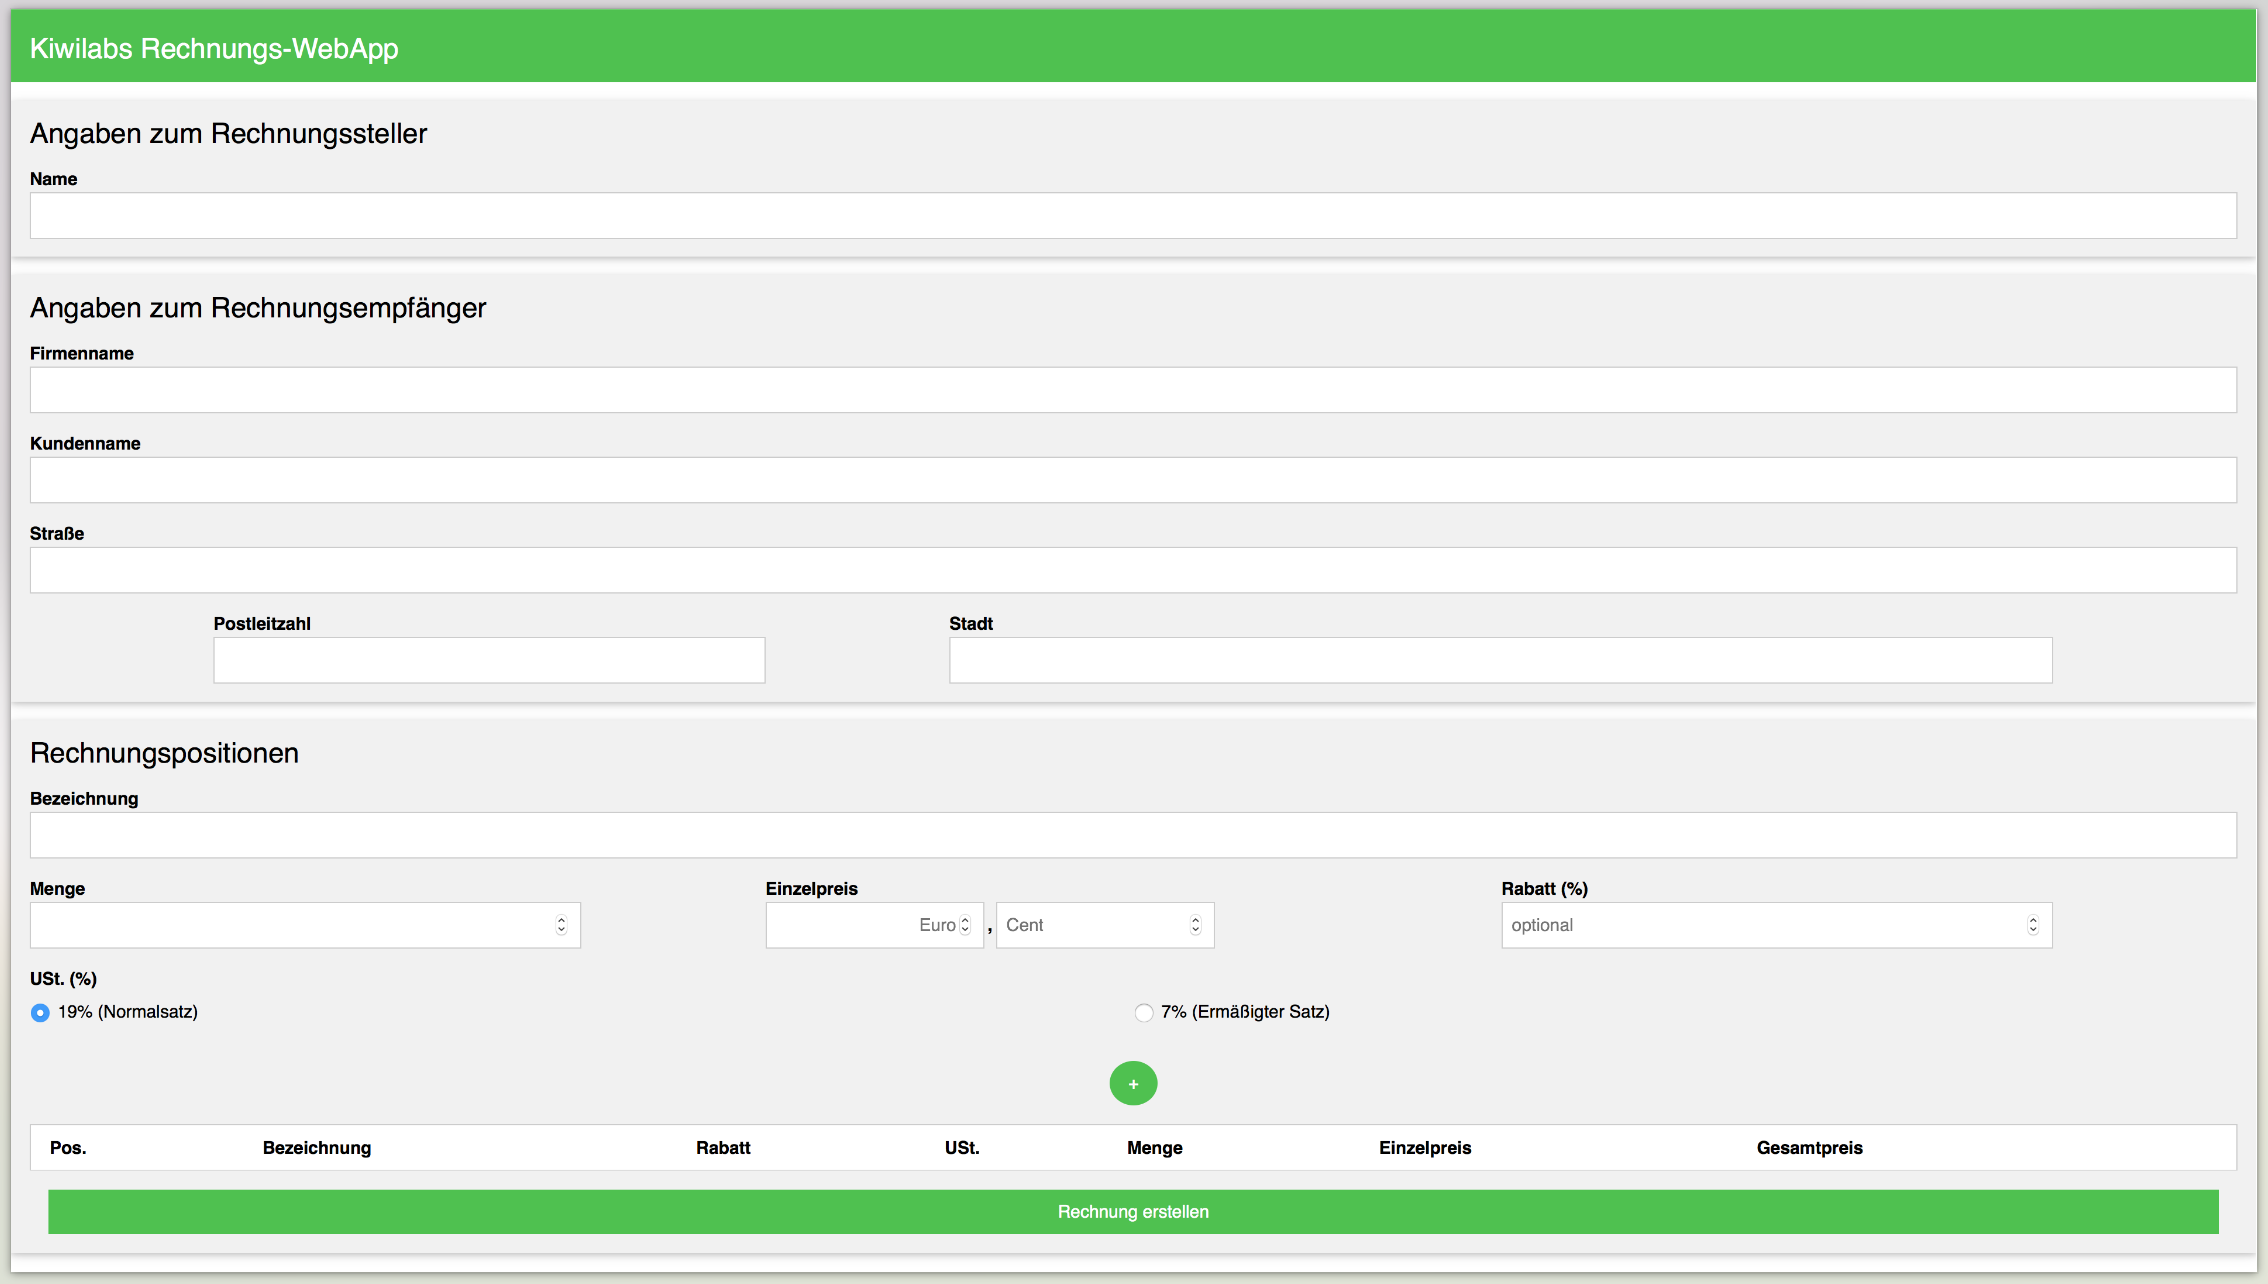
\includegraphics[width=1.0\textwidth]{imports/Layoutgesamt}
    \caption{Vollständiges Layout der Website}
\end{figure}
%
Ausgehend von den \ac{HTML}-Kenntnissen (siehe Seite \pageref{sec:HTML}) wird der \textit{Head} des Dokuments angelegt.
\lstinputlisting[language=HTML, firstline=1, lastline=14, firstnumber=1]{src/main.html} \label{Head} 

In Zeile 9 wird ein externes Stylesheet\cite{w3.css} eingebunden. Diese Vorlage ist lizenzfrei verfügbar von w3. Der \textit{Body} des HTML-Dokuments wird in Zeile 14 begonnen.\ref{Head}

\newpage
%%%%%%%%%%%%%%%%%%%%%%
\begin{description}
	\item[Angaben zum Rechnungssteller]
    \hfill
    \label{des:Angaben_Rechnungssteller}
\end{description}
%%%%%%%%%%%%%%%%%%%%%%
%
\lstinputlisting[language=HTML, firstline=22, lastline=39, firstnumber=22]{src/main.html}

In Zeile 22 wird ein neuer \textit{div}-Tag mit der Klasse \textit{w3-card} eröffnet. Dies ist eine Box mit Schatteneffekt. In Zeile 24 wird ein neuer div-Tag geöffnet, der ein Container mit einem Padding von 16 Pixel mit der Hintergrundfarbe von hellgrau darstellt. Dieses Element hat die schwarze Überschrift \textit{Angaben zum Rechnungssteller}. 
\begin{figure}[H]
    \centering
    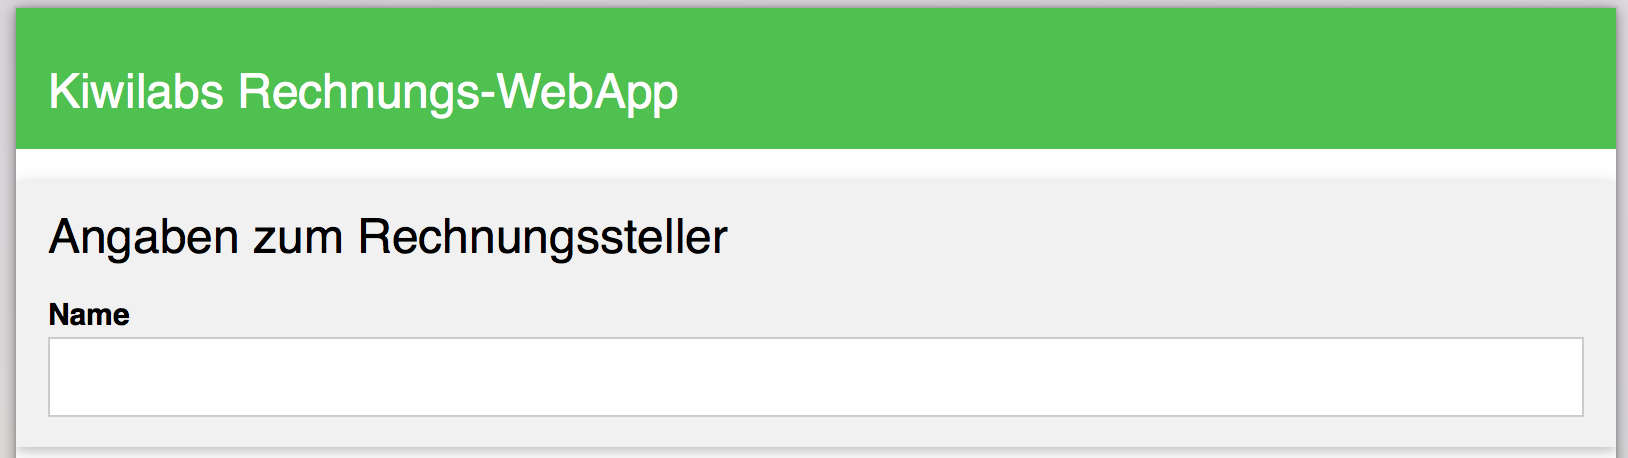
\includegraphics[width=0.7\textwidth]{imports/AzR}
    \caption{  Angaben zum Rechnungssteller}
  
\end{figure}
%
Ab Zeile 27 wird der Input beschrieben. Die darauf folgenden Attribute \textit{ng-click} und \textit{ng-model} sind Elemente von AngularJs, die die Reaktion der Eingabefelder gewährleisten. Dieser Punkt wird später näher beschrieben. \textit{w3-input} ist die Definition für einen Input und \textit{w3-border} sorgt für eine Umrandung des HTML-Elements. Zur korrekten Vervollständigung wurde außerdem eine ID, ein Name und ein Typ angegeben.
Der nächste Bereich, eingeleitet durch den Aufruf \textit{div} in Zeile 29, dient zur Implementierung des PopUp Effekts für eine Schnellauswahl der Rechnungssteller. Die Elemente dieser werden durch eine ungeordnete Liste, abgekürzt durch \textit{ul}, dargestellt. \textit{w3-hoverable} sorgt für die dynamische Hervorhebung des Namens, wenn die Maus des Nutzers über die Stelle fährt. 

\newpage
%%%%%%%%%%%%%%%%%%%%%%
\begin{description}
	\item[Angaben zum Rechnungsempfänger]
    \hfill
     \label{des:Angaben_Rechnungsempfänger}
\end{description}
%%%%%%%%%%%%%%%%%%%%%%
%
Die Layouterstellung des Abschnittes über die \textit{Angaben zum Rechnungsempfänger} sind analog zu \textit{Angaben zum Rechnungssteller}, weswegen nicht näher darauf eingegangen wird.


%%%%%%%%%%%%%%%%%%%%%%
\begin{description}
	\item[Darstellung der Rechnungspositionen]
    \hfill
    \label{des:Rechnungspositionen}
\end{description}
%%%%%%%%%%%%%%%%%%%%%%
%
Der Abschnitt zu den Rechnungspositionen wird in Zeile 88 begonnen. In Zeile 98 beginnt eine \textit{w3-row}. Diese sorgt für eine Reihung der Elemente \textit{Menge}, \textit{Einzelpreis} und \textit{Rabatt} nebeneinander. Für den Anwender soll das Layout nicht nur in der Ansicht eines Laptops oder PC, sondern auch in einer mobilen Version ansehnlich sein. Dies wird in Zeile 101 mittels der Klasse \textit{w3-col} gewährleistet. \textit{m3} definiert die Darstellung für alle Medium Geräte, diese sind bei \textit{w3school} größer als 601 Pixel. In dieser Darstellung nimmt es 3/12 der Bildschirmbreite ein. Ein Endgerät mit weniger als 601 Pixel Bildschirmbreite wird von \textit{w3.css} als \textit{small} bezeichnet. Dieses würde in diesem Fall das Element auf der gesamten Bildschirmbreite angezeigt bekommen. In Zeile 106 wird der Abstand zwischen den Feldern \textit{Menge} und \textit{Einzelpreis} bei großen Bildschirmen eingefügt. Der Aufruf \textit{w3-hide-small} entfernt den Abstand in der Ansicht von kleinen Bildschirmen.

\begin{figure}[H]
    \centering
    \begin{minipage}{0.45\linewidth}
        \centering
        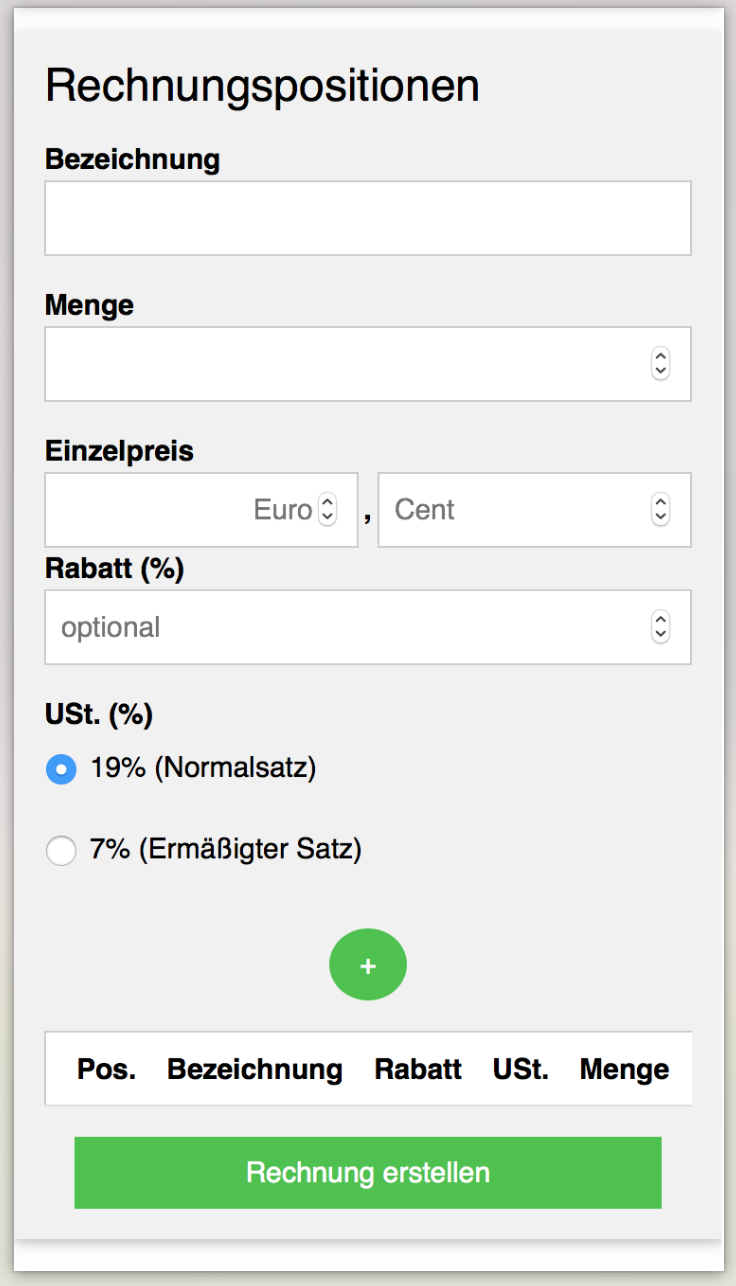
\includegraphics[width=0.33\textwidth]{imports/smallView}
        \caption{Mobile Ansicht}
    \end{minipage}
    %\hfill
    \begin{minipage}{0.45\linewidth}
        \centering
        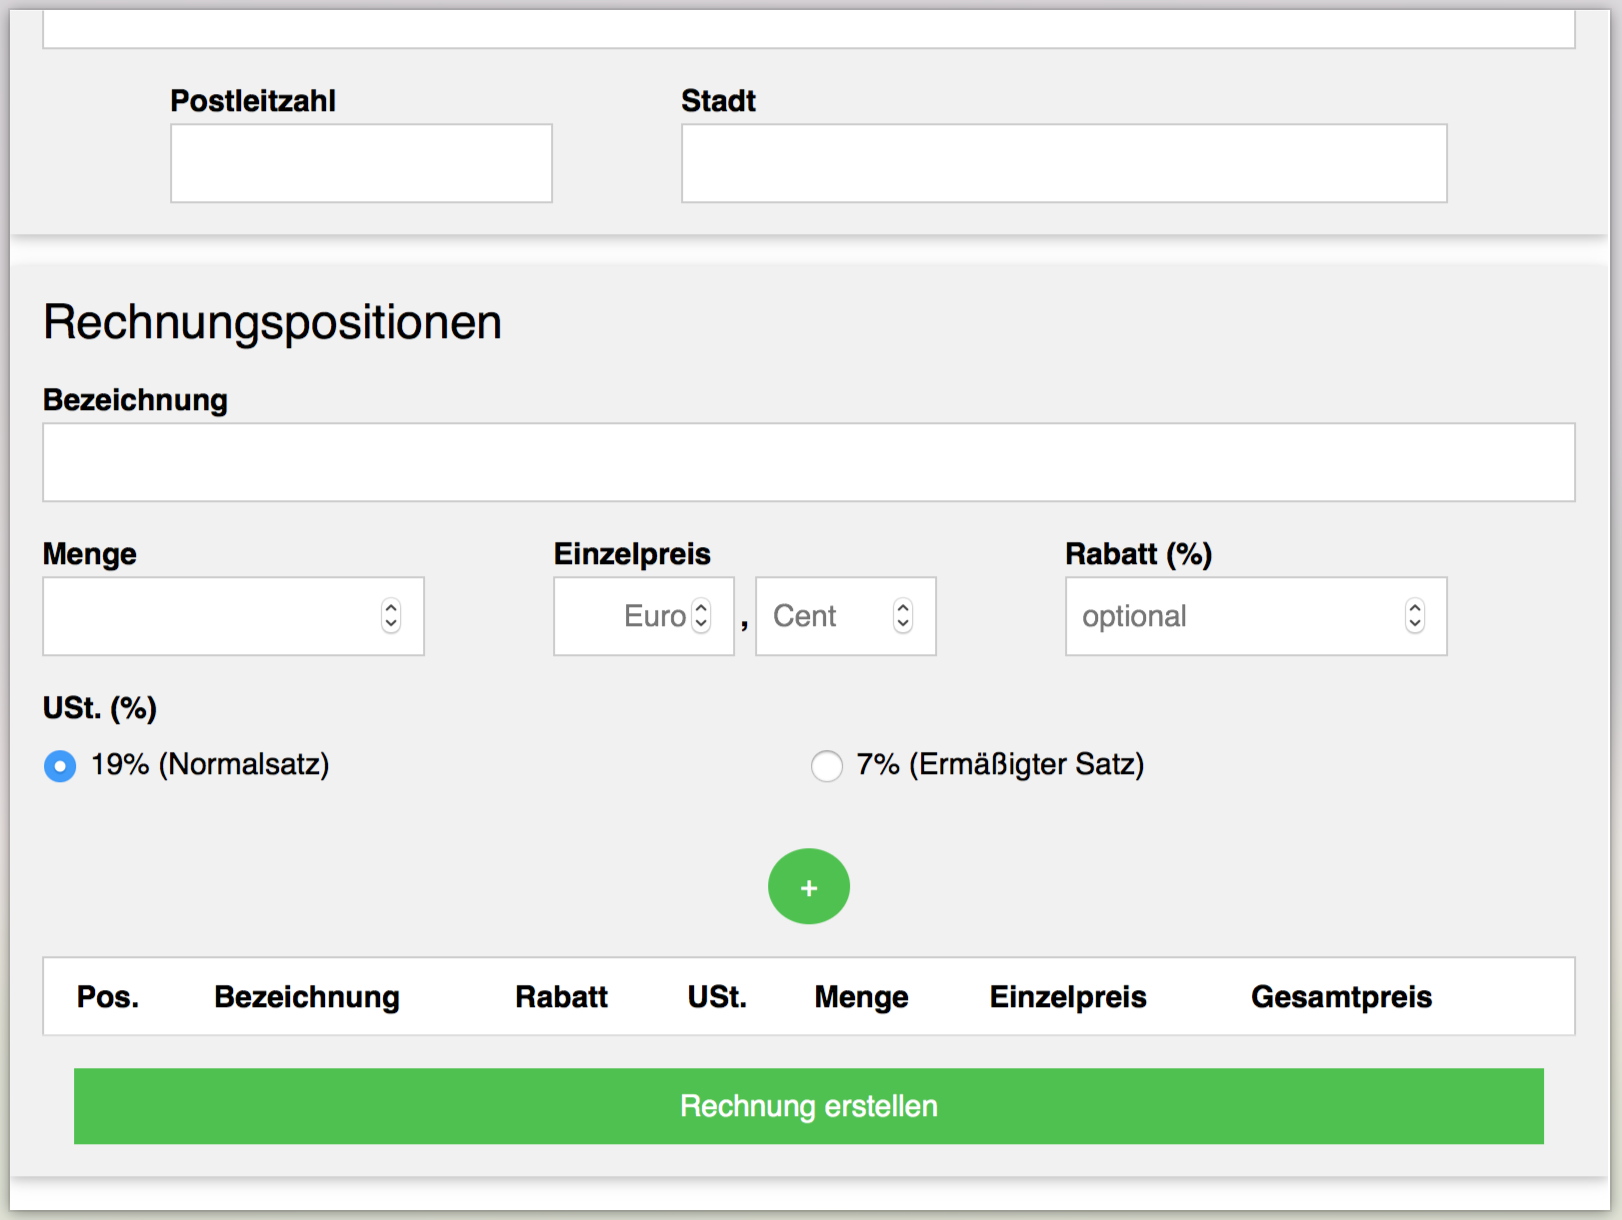
\includegraphics[width=0.8\textwidth]{imports/medium+largeView}
        \caption{Desktop Ansicht}
    \end{minipage}
\end{figure}

\lstinputlisting[language=HTML, firstline=88, lastline=108, firstnumber=88]{src/main.html}

Das Feld für den Einzelpreis wird ab Zeile 111 definiert, welches in Euro und Cent dargestellt werden soll, um den individuellen Kostenbetrag darstellen und eine weitere Verarbeitung des Betrages erreichen zu können. Wenn der Kostenbetrag mit Kommatrennung des Euro- und Centanteils in ein Feld geschrieben werden würde, müsste dieser mit einer Parse-Funktion eventuell später überarbeitet werden. Dieser Schritt wird durch eine explizite Trennung in zwei Eingabefelder eingespart. Diese beiden Felder werden jeweils durch eine \textit{w3-cell} definiert, diese ist ein einfaches und horizontal orientiertes Block-Element. 
Auf die Eingabefunktion und Übernahme des Betrages zu einem späteren Zeitpunkt eingegangen.

\lstinputlisting[language=HTML, firstline=111, lastline=129, firstnumber=111]{src/main.html}

Das nächste Feld der Rechnungspositionen ist der Rabatt, dies wird in der Zeile 132 begonnen und in Zeile 137 mit \bashCommand{</div>} beendet.

\lstinputlisting[language=HTML, firstline=132, lastline=137, firstnumber=132]{src/main.html}

Das letzte Element für die Rechnungspositionen ist die zu addierende Umsatz- und Mehrwertsteuer, die in der Preisberechnung berücksichtigt werden muss. 
Hier wird wieder eine \textit{w3-row} eröffnet, die mit USt. und 7 Prozent Ermäßigter Satz beschriftet wird. Dazwischen befinden sich Elemente, die durch AngularJs interaktiv auf den Nutzer der Website reagieren.

\lstinputlisting[language=HTML, firstline=141, lastline=152, firstnumber=141]{src/main.html}

Um weitere Positionen hinzufügen zu können, ist eine Add-Funktion gefordert, die benutzerfreundlich durch einen Plus-Button repräsentiert wird. 
%
Als letzter Punkt soll in der Ansicht der Website in einer Zeile alle Punkte der Rechnung übersichtlich dargestellt sein, was nun definiert wird. In Zeile 154 wird hierzu das Element in dem Zentrum des Bildschirms angeordnet. Innerhalb des \textit{ng-click} von AngularJS wird das Feld als runder Button mit grüner Füllung und automatisch berechnetem Abstand. 

\lstinputlisting[language=HTML, firstline=154, lastline=156, firstnumber=155]{src/main.html}

\begin{figure}[H]
    \centering
    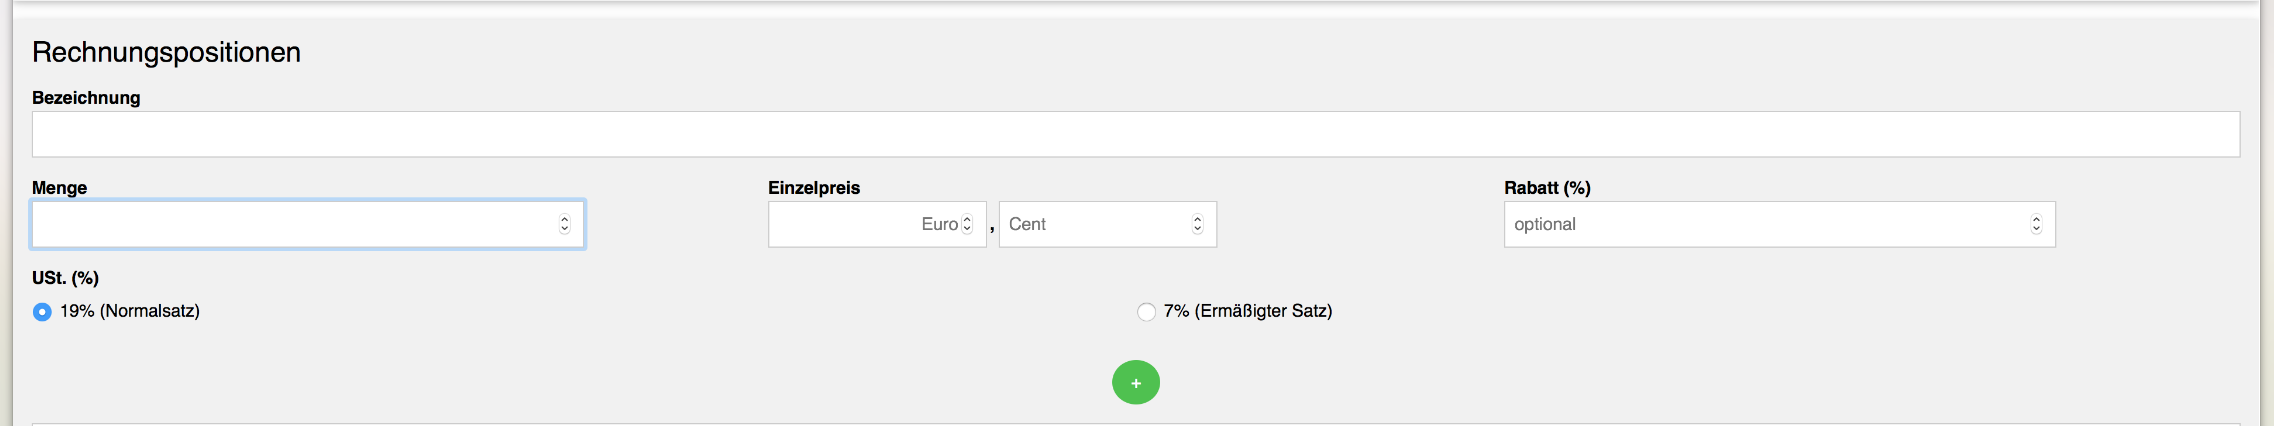
\includegraphics[width=0.7\textwidth]{imports/Rechnungspositonen}
    \caption{ Fertige Ansicht der Rechnungspositionen}
\end{figure}
%
Nun sind die benötigten Punkte der Rechnungspositonen komplettiert und zur Veranschaulichung der gesamten Rechnung werden am Ende des Websitenlayouts alle Teile in einer Reihe aufgeführt. 
\\

Für diese Anforderung wird eine Tabelle eröffnet, die sich dynamisch an die jeweilige Bildschirmgröße anpasst. ( \textit{w3-responsive, Z. 158f}. Die einzelnen Punkte werden in der Tabelle durch den \bashCommand{<t>} Tag in Zeile 160 und die jeweiligen \bashCommand{<th>} Tags als einzelne Elemente in einer neuen Zeile implementiert.

\lstinputlisting[language=HTML, firstline=158, lastline=182, firstnumber=158]{src/main.html}


%%%%%%%%%%%%%%%%%%%%%%
\begin{description}
	\item[Button für die Erstellung des Latex-Dokuments]
    \hfill
    \label{des:AddButton}
\end{description}
%%%%%%%%%%%%%%%%%%%%%%
%
Der Button für die Erstellung des Latex-Dokuments wird zentriert auf dem Display des Nutzers (vgl. Z.184 ) platziert. Außerdem ist der \textit{w3-button} ein grüner Block, weswegen er die gesamte Breite des Bildschirms benutzt und die Aufschrift \glqq{\textit{Rechnung erstellen}} trägt. Die Erstellung in ein pdf wird über AngularJs in \textit{Logik des Frontends} gewährleistet.



%%%%%%%%%%%%%%%%%%%%%%%%%%%%%%%%%%%%%%%%%%%%%%%%%%%%%%%%%%
%%%%%%%%%%				Logik					%%%%%%%%%%	
%%%%%%%%%%%%%%%%%%%%%%%%%%%%%%%%%%%%%%%%%%%%%%%%%%%%%%%%%%
\subsection{Logik des Frontends}
\label{sec:Logik}
%%%%%%%%%%%%%%%%%%%%%%%%%%%%%%%%%%%%%%%%%%%%%%%%%%%%%%%%%%


%%%%%%%%%%%%%%%%%%%%%%
\begin{description}
	\item[Logik für Rechnungssteller und -empfänger]
    \hfill
    \label{des:Logik}
\end{description}
%%%%%%%%%%%%%%%%%%%%%%
%
Die Logik des Frontends ist ein substantieller Teil der Websitencharaktertistik. Durch diese wird die Reaktion der Website auf Benutzereingaben oder Veränderungen der Fenstergröße garantiert. 
%
AngularJS wird das erste Mal in dem Projekt benötigt, wenn bei der Auswahl des Rechnungsstellers zwischen zuvor hinterlegten Personen gewählt werden soll, die als neue Option auf dem Desktop erscheinen sollen. Eine solche Interaktion wird in Zeile 27 durch den \textit{input}-Aufruf \textit{ng-click} und \textit{ng-model} implementiert.  Die erste Direktive teilt dem Java-Framework AngularJs mit, was bei einem Klick des Nutzers geschehen soll. Dies ist in diesem Fall \textit{toggleSenderList()}, diese Funktion wird in \textit{invoiceApp.js} definiert. Die Direktive \textit{ng-model} verbindet das Eingabefeld mit der in \textit{invoiceApp.js} definierten Variable\textit{senderName}. \textit{ng-show} ermöglicht die Darstellung der Sender Liste. Die Namen werden über die REST Schnittstelle im JSON Format übergeben und dienen der Vorauswahl. Wenn neue Namen eingeben werden, die noch nicht existent sind, werden diese an den Server übergeben und hinterlegt.
Die Logik für die Auswahl der Rechnungsempfänger\textit{(vgl. 48ff)} ist entsprechend diesem Prinzip. 

%%%%%%%%%%%%%%%%%%%%%%
\begin{description}
	\item[PDF-Erstellung]
    \hfill
    \label{sec:PDF}
\end{description}
%%%%%%%%%%%%%%%%%%%%%%
%
\lstinputlisting[language=HTML, firstline=184, lastline=186, firstnumber=183]{src/main.html}

In Zeile 185 des html-Dokuments wird mittels \textit{ng-click} mitgeteilt, dass bei einem Klick auf den Button \textit{downloadPDF} die gleichnamige, in \textit{invoiceApp.js} definierte Funktion ausgeführt werden soll. 
Diese legt das Objekt\textit{data} neu an und befüllt deren Variablen mit denen aus der Website. Im nächsten Schritt wird \textit{data} an den \textit{localhost} gepostet. Falls dies nicht funktioniert, wird die Nachricht "Fehler" gemeldet.

\lstinputlisting[language=JavaScript, firstline=79, lastline=99, firstnumber=79]{src/invoiceApp.js}


